\documentclass{report}
\usepackage[utf8]{inputenc}
\usepackage[italian]{babel}
\usepackage{float}
\usepackage{minted}
\usepackage[hidelinks]{hyperref}
\usepackage{titling}
\usepackage{titlesec}
\usepackage{listings}

% Language Definitions for SPARQL
%\lstset{language=SQL,morekeywords={PREFIX,java,rdf,rdfs,url}}

\lstset{
    language=SQL,
    morekeywords={PREFIX, java, rdf, rdfs, url},
    basicstyle=\ttfamily,
    frame=single,
    numbers=left,
    numberstyle=\tiny\color{black},
    keywordstyle=\color{blue},
    %keywordstyle=\color[rgb]{0.5, 0.5, 0},
    commentstyle=\color{gray},
    alsoletter={?},
    literate={?}{{\textcolor{red}{?}}}1,
    moredelim=[s][\color{purple}]{?}{\ },
    breaklines=true,
}

\setlength{\droptitle}{-15em}   % This is your set screw

%%%%%%%%%%%%%%%%%%%%%%%%%%%%%%%%%%%%%%%%%
% Lachaise Assignment
% Structure Specification File
% Version 1.0 (26/6/2018)
%
% This template originates from:
% http://www.LaTeXTemplates.com
%
% Authors:
% Marion Lachaise & François Févotte
% Vel (vel@LaTeXTemplates.com)
%
% License:
% CC BY-NC-SA 3.0 (http://creativecommons.org/licenses/by-nc-sa/3.0/)
% 
%%%%%%%%%%%%%%%%%%%%%%%%%%%%%%%%%%%%%%%%%

%----------------------------------------------------------------------------------------
%	PACKAGES AND OTHER DOCUMENT CONFIGURATIONS
%----------------------------------------------------------------------------------------

\usepackage{amsmath,amsfonts,stmaryrd,amssymb} % Math packages

\usepackage{enumerate} % Custom item numbers for enumerations
\usepackage{titlesec}

\usepackage[ruled]{algorithm2e} % Algorithms

\usepackage[framemethod=tikz]{mdframed} % Allows defining custom boxed/framed environments

\usepackage{listings} % File listings, with syntax highlighting
\lstset{
	basicstyle=\ttfamily, % Typeset listings in monospace font
}

%----------------------------------------------------------------------------------------
%	DOCUMENT MARGINS
%----------------------------------------------------------------------------------------

\usepackage{geometry} % Required for adjusting page dimensions and margins

\geometry{
	paper=a4paper, % Paper size, change to letterpaper for US letter size
	top=2.5cm, % Top margin
	bottom=3cm, % Bottom margin
	left=2.5cm, % Left margin
	right=2.5cm, % Right margin
	headheight=14pt, % Header height
	footskip=1.5cm, % Space from the bottom margin to the baseline of the footer
	headsep=1.2cm, % Space from the top margin to the baseline of the header
	%showframe, % Uncomment to show how the type block is set on the page
}

%----------------------------------------------------------------------------------------
%	FONTS
%----------------------------------------------------------------------------------------

\usepackage[utf8]{inputenc} % Required for inputting international characters
\usepackage[T1]{fontenc} % Output font encoding for international characters

\usepackage{XCharter} % Use the XCharter fonts

\DeclareOldFontCommand{\bf}{\normalfont\bfseries}{\mathbf}

%----------------------------------------------------------------------------------------
%	COMMAND LINE ENVIRONMENT
%----------------------------------------------------------------------------------------

% Usage:
% \begin{commandline}
%	\begin{verbatim}
%		$ ls
%		
%		Applications	Desktop	...
%	\end{verbatim}
% \end{commandline}

\mdfdefinestyle{commandline}{
	leftmargin=10pt,
	rightmargin=10pt,
	innerleftmargin=15pt,
	middlelinecolor=black!50!white,
	middlelinewidth=2pt,
	frametitlerule=false,
	backgroundcolor=black!5!white,
	frametitle={Command Line},
	frametitlefont={\normalfont\sffamily\color{white}\hspace{-1em}},
	frametitlebackgroundcolor=black!50!white,
	nobreak,
}

% Define a custom environment for command-line snapshots
\newenvironment{commandline}{
	\medskip
	\begin{mdframed}[style=commandline]
}{
	\end{mdframed}
	\medskip
}

%----------------------------------------------------------------------------------------
%	FILE CONTENTS ENVIRONMENT
%----------------------------------------------------------------------------------------

% Usage:
% \begin{file}[optional filename, defaults to "File"]
%	File contents, for example, with a listings environment
% \end{file}

\mdfdefinestyle{file}{
	innertopmargin=1.6\baselineskip,
	innerbottommargin=0.8\baselineskip,
	topline=false, bottomline=false,
	leftline=false, rightline=false,
	leftmargin=2cm,
	rightmargin=2cm,
	singleextra={%
		\draw[fill=black!10!white](P)++(0,-1.2em)rectangle(P-|O);
		\node[anchor=north west]
		at(P-|O){\ttfamily\mdfilename};
		%
		\def\l{3em}
		\draw(O-|P)++(-\l,0)--++(\l,\l)--(P)--(P-|O)--(O)--cycle;
		\draw(O-|P)++(-\l,0)--++(0,\l)--++(\l,0);
	},
	nobreak,
}

% Define a custom environment for file contents
\newenvironment{file}[1][File]{ % Set the default filename to "File"
	\medskip
	\newcommand{\mdfilename}{#1}
	\begin{mdframed}[style=file]
}{
	\end{mdframed}
	\medskip
}

%----------------------------------------------------------------------------------------
%	NUMBERED QUESTIONS ENVIRONMENT
%----------------------------------------------------------------------------------------

% Usage:
% \begin{question}[optional title]
%	Question contents
% \end{question}

\mdfdefinestyle{question}{
	innertopmargin=1.2\baselineskip,
	innerbottommargin=0.8\baselineskip,
	roundcorner=5pt,
	nobreak,
	singleextra={%
		\draw(P-|O)node[xshift=1em,anchor=west,fill=white,draw,rounded corners=5pt]{%
		\questionTitle};
	},
}

\newcounter{Question} % Stores the current question number that gets iterated with each new question

% Define a custom environment for numbered questions
\newenvironment{question}[1][\unskip]{
	\bigskip
	\stepcounter{Question}
	\newcommand{\questionTitle}{~#1}
	\begin{mdframed}[style=question]
}{
	\end{mdframed}
	\medskip
}

%----------------------------------------------------------------------------------------
%	WARNING TEXT ENVIRONMENT
%----------------------------------------------------------------------------------------

% Usage:
% \begin{warn}[optional title, defaults to "Warning:"]
%	Contents
% \end{warn}

\mdfdefinestyle{warning}{
	topline=false, bottomline=false,
	leftline=false, rightline=false,
	nobreak,
	singleextra={%
		\draw(P-|O)++(-0.5em,0)node(tmp1){};
		\draw(P-|O)++(0.5em,0)node(tmp2){};
		\fill[black,rotate around={45:(P-|O)}](tmp1)rectangle(tmp2);
		\node at(P-|O){\color{white}\scriptsize\bf !};
		\draw[very thick](P-|O)++(0,-1em)--(O);%--(O-|P);
	}
}

% Define a custom environment for warning text
\newenvironment{warn}[1][Warning:]{ % Set the default warning to "Warning:"
	\medskip
	\begin{mdframed}[style=warning]
		\noindent{\textbf{#1}}
}{
	\end{mdframed}
}

%----------------------------------------------------------------------------------------
%	INFORMATION ENVIRONMENT
%----------------------------------------------------------------------------------------

% Usage:
% \begin{info}[optional title, defaults to "Info:"]
% 	contents
% 	\end{info}

\mdfdefinestyle{info}{%
	topline=false, bottomline=false,
	leftline=false, rightline=false,
	nobreak,
	singleextra={%
		\fill[black](P-|O)circle[radius=0.4em];
		\node at(P-|O){\color{white}\scriptsize\bf i};
		\draw[very thick](P-|O)++(0,-0.8em)--(O);%--(O-|P);
	}
}

% Define a custom environment for information
\newenvironment{info}[1][Info:]{ % Set the default title to "Info:"
	\medskip
	\begin{mdframed}[style=info]
		\noindent{\textbf{#1}}
}{
	\end{mdframed}
}



\titleclass{\subsubsubsection}{straight}[\subsection]

\newcounter{subsubsubsection}[subsubsection]
\renewcommand\thesubsubsubsection{\thesubsubsection.\arabic{subsubsubsection}}
\renewcommand\theparagraph{\thesubsubsubsection.\arabic{paragraph}} % optional; useful if paragraphs are to be numbered

\titleformat{\subsubsubsection}
  {\normalfont\normalsize\bfseries}{\thesubsubsubsection}{1em}{}
\titlespacing*{\subsubsubsection}
{0pt}{3.25ex plus 1ex minus .2ex}{1.5ex plus .2ex}

\makeatletter
\renewcommand\paragraph{\@startsection{paragraph}{5}{\z@}%
  {3.25ex \@plus1ex \@minus.2ex}%
  {-1em}%
  {\normalfont\normalsize\bfseries}}
\renewcommand\subparagraph{\@startsection{subparagraph}{6}{\parindent}%
  {3.25ex \@plus1ex \@minus .2ex}%
  {-1em}%
  {\normalfont\normalsize\bfseries}}
\def\toclevel@subsubsubsection{4}
\def\toclevel@paragraph{5}
\def\toclevel@paragraph{6}
\def\l@subsubsubsection{\@dottedtocline{4}{7em}{4em}}
\def\l@paragraph{\@dottedtocline{5}{10em}{5em}}
\def\l@subparagraph{\@dottedtocline{6}{14em}{6em}}
\makeatother

\setcounter{secnumdepth}{4}
\setcounter{tocdepth}{4}


\title{
    \Huge Motology\\
    \Large Motorsports championship Ontology\\ 
    \Large Relazione Web Semantico
}

\author{Serafini Andrea, Sanchi Piero}

\usepackage{natbib}
\bibliographystyle{unsrt}
\usepackage{graphicx}

\usepackage{tabularx}
\usepackage[justification=centering]{caption}
\usepackage{minted}
\usemintedstyle{vs}
\definecolor{bg}{rgb}{0.95,0.95,0.95}

\titleformat{\chapter}[display]   
{\normalfont\huge\bfseries}{\chaptertitlename\ \thechapter}{20pt}{\Huge}   
\titlespacing*{\chapter}{0pt}{-20pt}{20pt}

\begin{document}

\maketitle

\tableofcontents
\listoffigures

\chapter{Dominio del progetto}

\section{Introduzione}
Motology è un ontologia riguardante il mondo delle competizioni motociclistiche, improntata particolarmente sul Motomondiale. Nasce con lo scopo di aiutare appassionati, meccanici, piloti, cronisti etc. ad ottenere informazioni e statistiche composite riguardanti il loro sport preferito. L'ontologia nasce a scopo consultativo, tuttavia potenzialmente potrebbe essere impiegata per derivare nuovi dati o studiare correlazioni ed allenare modelli di intelligenza artificiale a prevedere trend futuri. 
\\\\
La prima fase della modellazione ha coinvolto la definizione di tutte le entità che compongono l'ontologia, partendo dalle classi, proprietà e vincoli. In una seconda fase dopo aver verificato che il sistema inferisse nuove informazioni da ciò che era stato definito, sono state formulate diverse query in modo da mostrare le potenzialità dell'ontologia e da ottenere informazioni derivate in modo semplice, senza dover svolgere numerose ricerche online dovendosi trovare ad unificare dati sparsi ed eterogenei. L'immagine seguente riassume brevemente l'ordine di grandezza di Motology:
\\
\begin{figure}[H]
    \begin{center}
        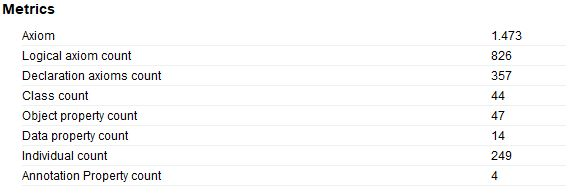
\includegraphics[scale=0.9]{img/statistiche.jpg}
       \caption{Un pò di numeri riguardanti Motology} 
    \end{center}
\end{figure}

In seguito illustreremo le classi principali, citeremo le ontologie esterne impiegate per modellare determinati concetti di natura più generale rispetto al dominio in oggetto ed infine faremo una panoramica delle tecnologie adottate per lo sviluppo di Motology.

\newpage

\section{Design: scelta delle Classi}
Nella prima parte della definizione dell'ontologia è stato fondamentale delineare il "perimetro" ed il livello di dettaglio di cui dotare Motology allo scopo di non trattare determinati temi in maniera troppo approfondita per mantenere solamente dati utili a formare interrogazioni interessanti. Le classi che ci hanno aiutato a definire questi aspetti sono state:

\subsection{moto:GranPremio}
Classe che rappresenta (da wikipedia) "un insieme di gare di velocità su pista delle due ruote motorizzate che si svolge su un apposito circuito", nonchè il soggetto principale di Motology. La peculiarità di un gran premio motociclistico è che si svolge in un singolo circuito per ogni nazione (es. Mugello per il gran premio d'Italia), comprende tutte le competizioni, gare, qualifiche e prove libere, per ogni campionato (es. Moto2, MotoGP). Nel successivo capitolo spiegheremo più in dettaglio come sono stati modellati tutti questi concetti, partendo da quello di Gran Premio. Di seguito possiamo vedere come risulta la struttura finale dell'ontologia:
\\\\
\begin{figure}[H]
    \begin{center}
        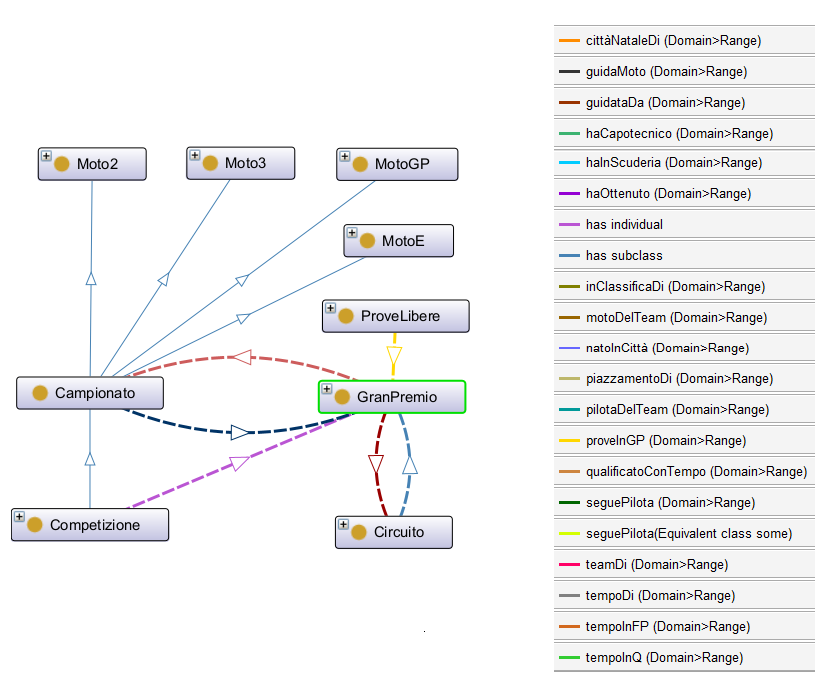
\includegraphics[scale=0.9]{img/gran premio.png}
       \caption{Ontograph riguardante il Gran Premio} 
    \end{center}
\end{figure}

\newpage

\subsection{moto:Pilota}
 La scelta di creare una classe separata per i piloti è stata motivata dalla necessità di modellare una componente fondamentale di un evento motociclistico, la presenza di un protagonista, delineato appunto da Pilota. Questa classe, oltre a consentire di specificare attributi e relazioni uniche per questo ruolo specifico, ci ha permesso di riflettere sugli altri ruoli della "Persona" all'interno di questo ambito. Abbiamo quindi deciso di modellare il concetto di Persona, andando a riutilizzare la definizione presente in FOAF per modellare anche altre figure, come quelle di Capo tecnico, Team Manager, ed alcuni casi particolari di pilota detti "Leggende" (coloro che hanno vinto almeno un gran premio per ogni campionato). Queste figure saranno spiegate in maggior dettaglio nel capitolo successivo.
\\\\
\begin{figure}[H]
    \begin{center}
        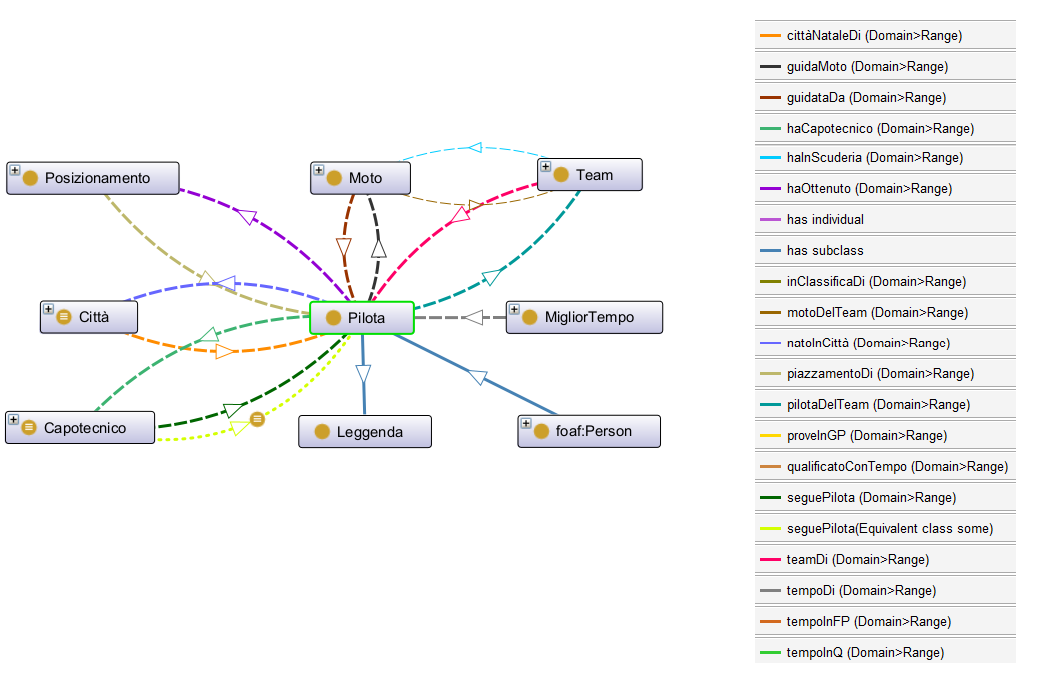
\includegraphics[scale=0.75]{img/pilota.png}
       \caption{Ontograph riguardante il Pilota} 
    \end{center}
\end{figure}

\newpage

\subsection{moto:Moto}
Ulteriore aspetto che abbiamo ritenuto fondamentale per ottenere statistiche e recommendation esaustive (oltre all'evento "Gran Premio" e la persona "Pilota") è quello del veicolo impiegato in questo tipo di competizioni, la Moto. Le moto da gran premio sono prototipi da competizione, sviluppate specificamente per le corse e non sono disponibili sul mercato. Questa classe ci permette di scendere nei dettagli più tecnici ed eventualmente di rendere estendibile Motology da chiunque volesse modellare scelte dello staff ingegneristico (ad esempio la scelta delle gomme basata sulle condizioni climatiche e meteorologiche). Analizzando questa classe e le sue proprietà in fase di progettazione abbiamo deciso di modellare altri concetti strettamente collegati a quello di moto, come il tipo di motore ed alcune sue caratteristiche e l'azienda produttrice del prototipo, che coincide spesso con la scuderia della moto.
    
\begin{figure}[H]
    \begin{center}
        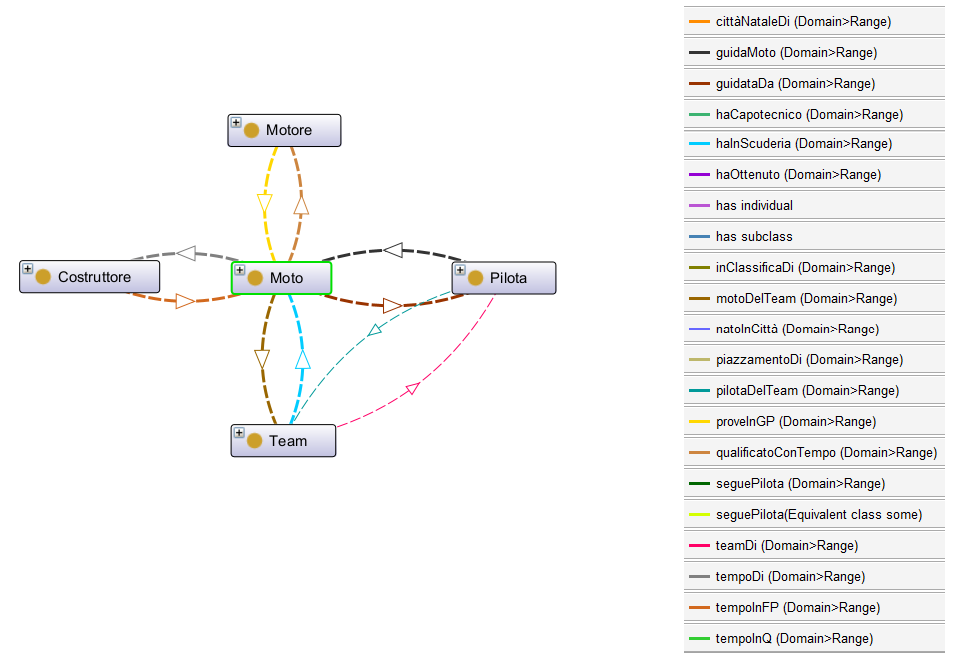
\includegraphics[scale=0.8]{img/moto.png}
       \caption{Ontograph riguardante la Moto} 
    \end{center}
\end{figure}

\newpage

\section{Impiego di ontologie esistenti}
Le Ontologie impiegate all'intero di questo progetto per modellare concetti già noti e ampiamente trattati sono:

\begin{itemize}
    \item \textbf{foaf:person} il motivo principale di questa scelta è stato quello di sfruttare la ricchezza concettuale offerta da FOAF (acronimo di Friend Of A Friend) per rappresentare le informazioni relative agli individui coinvolti nel contesto di Motology, tra cui troviamo i piloti, i capi tecnici ed i team manager. Questa scelta di integrazione tra Motology e FOAF ci consente di beneficiare dell'interoperabilità con altre ontologie e applicazioni semantiche che fanno uso di FOAF come standard per la rappresentazione delle informazioni personali e sociali.

    \item \textbf{dbo:nation e dbo:city} L'integrazione delle ontologie dbo:nation e dbo:city in Motology è stata effettuata per consentirci di modellare in modo completo e accurato informazioni di natura geografica coinvolte nel nostro sistema. Questa scelta è motivata dalla necessità di rappresentare proprietà come la nazionalità dei piloti, dei costruttori, il luogo in cui è presente un circuito e le località delle gare.
\end{itemize}

\section{Tecnologie e linguaggi adottati}
I vincoli implementativi hanno influenzato l'intero processo di realizzazione del sistema, determinando l'adozione di determinati linguaggi di programmazione e/o strumenti software specifici. Nel contesto dello sviluppo di questo progetto, ci siamo uniformati ad i seguenti vincoli tecnologici:

\begin{itemize}
    \item \textbf{RDF, RDF Schema e OWL:} Queste tecnologie sono state utilizzate per modellare il dominio del sistema. L'adozione di RDF (Resource Description Framework), RDF Schema e OWL (Web Ontology Language) ci ha permesso di rappresentare in modo strutturato e semantico le informazioni del dominio.
    \item \textbf{SPARQL:} Abbiamo adottato SPARQL come linguaggio di interrogazione all'ontologia. SPARQL ci consente di formulare query ottenendo risultati pertinenti in base alle nostre esigenze.
    \item \textbf{SWRL:} abbiamo impiegato SWRL (Semantic Web Rule Language) per esprimere regole di logica aggiuntive, come regole di inferenza che hanno permesso di dedurre nuove informazioni a partire dai dati esistenti nell'ontologia. Questo ha reso possibile l'applicazione di ragionamenti automatizzati e l'estensione delle capacità di inferenza del nostro sistema.
\end{itemize}
\chapter{Architettura dell'ontologia}
In questo capitolo illustreremo più in dettaglio la struttura e le scelte progettuali adottate per la creazione di Motology, partendo dalle classi, proprietà e data properties utilizzate, terminando con le regole SWRL.

\section{Specifiche dell'ontologia}
\begin{figure}[H]
    \begin{center}
        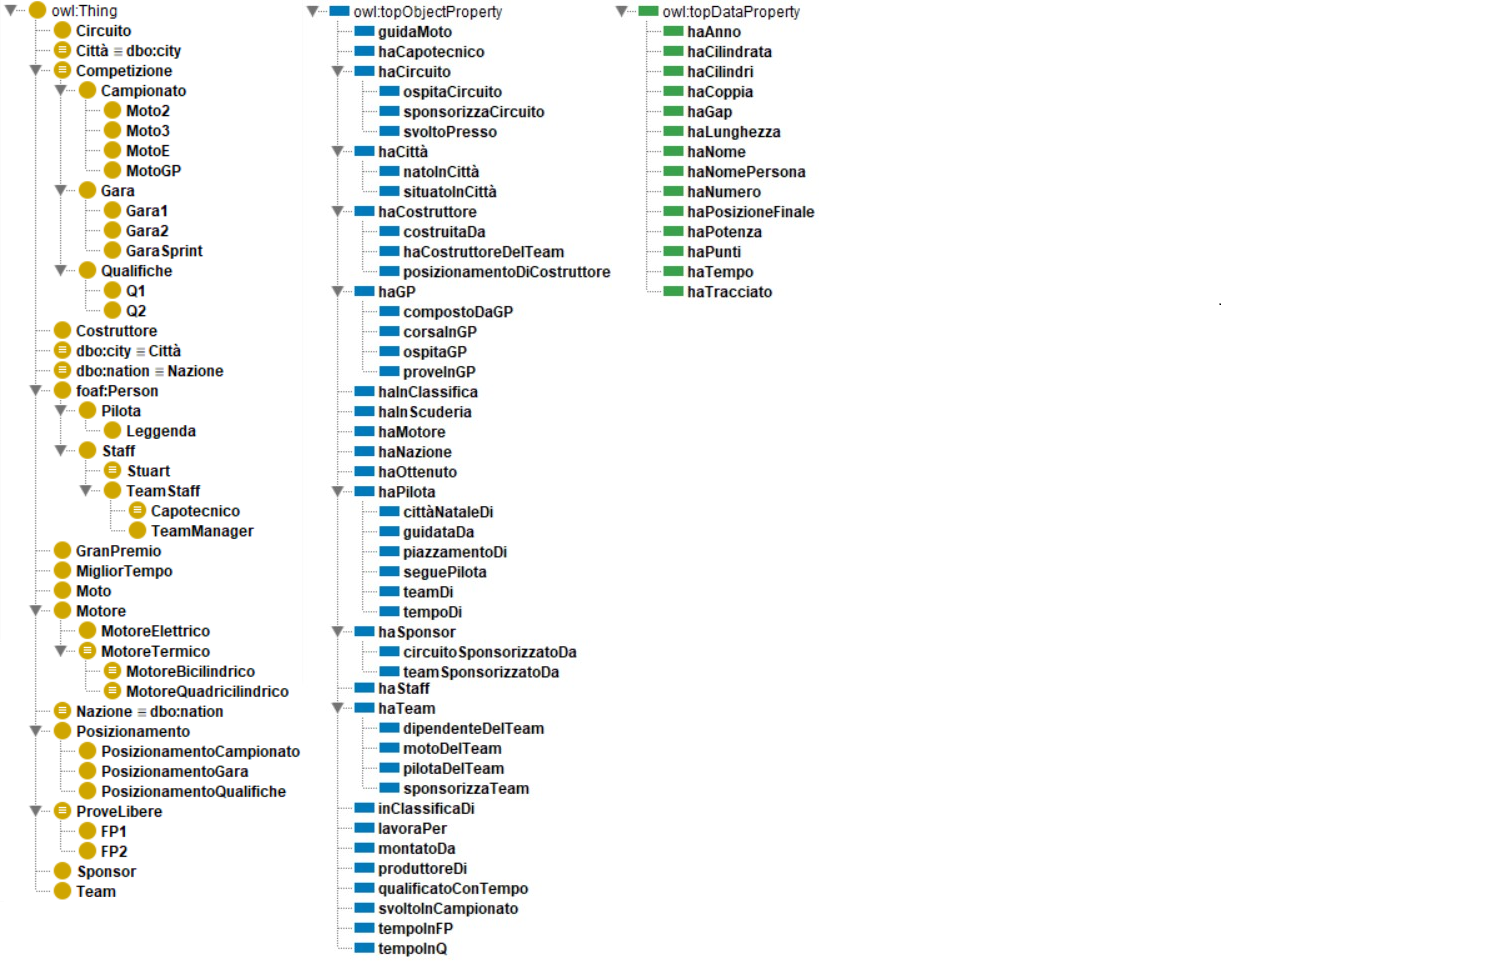
\includegraphics[scale=0.83]{img/Gerarchie.png}
       \caption{Totalità delle Classi, Object Properties e Data Properties.} 
    \end{center}
\end{figure}

\subsection{Classi}
Dopo la panoramica nel capitolo precedente dove sono state spiegte le classi principali, scenderemo più nel dettaglio riportando una spiegazione sintetica per ognuna della 44 classi che formano Motology.

\begin{itemize}
  \item \textbf{Città}: Rappresenta una città, come "insediamento umano di grandi dimensioni" (DBPedia).
  \item \textbf{Nazione}: Rappresenta una nazione, "comunità stabile di persone" (DBPedia).
  \item \textbf{Competizione}: Rappresenta un qualunque evento competitivo che vede come risultato una classifica, ha come sottoclassi Campionato, Gara e Sessione di Qualifica.
  \item \textbf{Campionato}: Rappresenta un campionato, a sua volta suddiviso in "classi" contraddistinte dalle caratteristiche delle moto che vi partecipano (es. Campionato di Moto2).
  \item \textbf{Moto2}: Rappresenta il campionato Moto2, contraddistinto da motori fino a 765 cm³ a quattro tempi fornito a tutte le squadre dalla stessa casa costruttrice.
  \item \textbf{Moto3}: Rappresenta il campionato Moto2, contraddistinto da motori fino a 250 cm³ a quattro tempi monocilindrici.  
  \item \textbf{MotoE}: Rappresenta il campionato MotoE, contraddistinto da prototipi a motore elettrico e alimentazione a batteria, il campionato più giovane nato nel 2019.
  \item \textbf{MotoGP}: Rappresenta il campionato MotoGP, contraddistinto da motori fino a 1000 cm³ a quattro tempi. \\ Per ogni campionato negli scorsi anni sono cambiate numerose volte le specifiche delle moto, inoltre negli anni anche i campionati sono notevolmente cambiati (seguendo il progresso tecnologico e l'attenzione all'ambiente). Motology per come è strutturata permette di modellare agilmente questi cambiamenti nel tempo.
  \item \textbf{Gara}: Rappresenta una singola gara di uno specifico campionato in uno specifico gran premio.
  \item \textbf{Gara1}: Nel caso di alcuni specifici campionati che la prevedono, rappresenta la prima gara di un Gran Premio.
  \item \textbf{Gara2}: Nel caso di alcuni specifici campionati che la prevedono, rappresenta la seconda gara di un Gran Premio
  \item \textbf{GaraSprint}: Nel caso di alcuni specifici campionati che la prevedono, rappresenta una gara speciale di un Gran Premio contraddistinta da meno giri.
  \item \textbf{Qualifiche}: Rappresenta una sessione di qualifica, competizione che permette di determinare le posizioni di partenza per una gara.
  \item \textbf{Q1}: Rappresenta la prima sessione di qualifica.
  \item \textbf{Q2}: Rappresenta la seconda sessione di qualifica.
  \item \textbf{Circuito}: Rappresenta una pista chiusa adibita a gare (anche di natura differente da quelle del motomondiale).
  \item \textbf{Costruttore}: Rappresenta il brand di un'azienda che costruisce prototipi da corsa.
  \item \textbf{ProveLibere}: Rappresenta le sessioni di prove libere prima di una gara.
  \item \textbf{FP1}: Rappresenta la prima sessione di prove libere.
  \item \textbf{FP2}: Rappresenta la seconda sessione di prove libere.
  \item \textbf{GranPremio}: Rappresenta un Gran Premio, evento cardine del motomondiale che contraddistingue tutte le competizioni che avverranno in uno specifico circuito (uno per stato, per questo diremo "Gran Premio d'Italia per indicare l'insieme delle competizioni svolte nel circuito del Mugello).
  \item \textbf{MigliorTempo}: Rappresenta il miglior tempo registrato da un partecipante in una competizione o in una prova libera.
  \item \textbf{Moto}: Rappresenta un prototipo da gara di un motociclo, veicolo a motore dotato di due ruote.
  \item \textbf{Motore}: Rappresenta un propulsore.
  \item \textbf{MotoreElettrico}: Rappresenta un motore elettrico (con caratteristiche legate ad emissioni e alimentazione molto differenti da motori termici).
  \item \textbf{MotoreTermico}: Rappresenta un motore a combustione interna.
   \begin{figure}[H]
    \begin{center}
        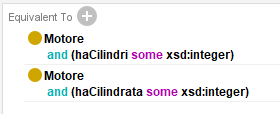
\includegraphics[scale=1]{img/spec_motoretermico.png}
       \caption{Modellazione motore termico.} 
    \end{center}
\end{figure}
  \item \textbf{MotoreBicilindrico}: Rappresenta un motore dotato di due cilindri.
  \begin{figure}[H]
    \begin{center}
        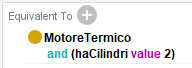
\includegraphics[scale=1]{img/spec_bicilindrico.png}
       \caption{Modellazione motore bicilindrico.} 
    \end{center}
\end{figure}
  \item \textbf{MotoreQuadricilindrico}: Rappresenta un motore dotato di quattro cilindri (che possono essere disposti seguendo diverse configurazioni).
    \begin{figure}[H]
    \begin{center}
        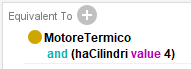
\includegraphics[scale=1]{img/spec_quadricilindrico.png}
       \caption{Modellazione motore quadricilindrico.} 
    \end{center}
\end{figure}
  \item \textbf{Posizionamento}: Rappresenta il risultato ottenuto dai partecipanti ad una gara (va a formare la classifica).
  \item \textbf{PosizionamentoCampionato}: Rappresenta il risultato ottenuto dai partecipanti al campionato (ottenuto applicando particolari criteri ai risultati delle singole gare e delle qualifiche).
  \item \textbf{PosizionamentoGara}: Rappresenta il posizionamento in una gara.
  \item \textbf{PosizionamentoQualifiche}: Rappresenta il risultato ottenuto dai partecipanti ad una sessione di qualifica.
  \item \textbf{Sponsor}: Rappresenta un'azienda, che fornisce supporto finanziario a una squadra o a un evento.
  \item \textbf{Team}: Rappresenta un team, che è composto da individui che competono insieme nel motomondiale.
  \item \textbf{Person}: Rappresenta un individuo.
  \item \textbf{Pilota}: Rappresenta l'individuo che conduce la moto in una gara motociclistica.
  \item \textbf{Leggenda}: Rappresenta un pilota che ha vinto almeno un campionato in ognuna delle tre categorie principali (Moto2, Moto3 e MotoGP), es. Valentino Rossi.
  \item \textbf{Staff}: Rappresenta membri dello staff coinvolti nel motomondiale.
  \item \textbf{Stuart}: Rappresenta un membro dello staff che lavora per uno specifico circuito.
    \begin{figure}[H]
    \begin{center}
        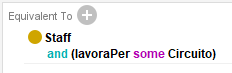
\includegraphics[scale=1]{img/spec_stuart.png}
       \caption{Modellazione stuart.} 
    \end{center}
\end{figure}
  \item \textbf{TeamStaff}: Rappresenta membri dello staff che lavorano per un team.
  \item \textbf{TeamManager}: Rappresenta un team manager, che è responsabile della gestione del team.
  \item \textbf{Capotecnico}: Individuo responsabile della gestione del team di meccanici e fautore delle decisioni tecniche.
    \begin{figure}[H]
    \begin{center}
        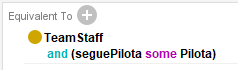
\includegraphics[scale=1]{img/spec_capotecnico.png}
       \caption{Modellazione capotecnico.} 
    \end{center}
\end{figure}
\end{itemize}

\subsection{Proprietà}
Le object properties rappresentano relazioni tra oggetti all'interno di uno dominio specifico. Nel nostro caso consentono di definire connessioni utili al processo di reasoning per inferire nuove informazioni ed utili all'ottenimento di statistiche composite per ognuna delle diverse entità che compongono Motology. 
Nella seguente sezione, vengono presentate proprietà utilizzate nel sistema, coadiuvate di una breve spiegazione per ciascuna di esse.

\begin{itemize}
    \item \textbf{guidaMoto}: Indica che un pilota guida una moto.
    \item \textbf{haCapotecnico}: Indica che un pilota fa riferimento ad un capo tecnico.
    
\item \textbf{haCircuito}: Indica che un soggetto ha un circuito associato.
    \item \textbf{ospitaCircuito}: Indica che una città ospita un circuito.
    \item \textbf{sponsorizzaCircuito}: Indica che uno sponsor (anche eventualmente un costruttore) finanzia un circuito ottenendo indietro pubblicità.
    \item \textbf{svoltoPresso}: Indica che un gran premio si svolge presso un circuito, questa proprità ne presuppone altre in quanto ogni nazione vede lo svolgersi di un gran premio in un solo circuito.
	
	\item \textbf{haCittà}: Indica che un soggetto è nato o situato in una specifica città.
    \item \textbf{natoInCittà}: Indica che un individuo è nato in una specifica città.
    \item \textbf{situatoInCittà}: Indica che un circuito è situato in una città.
	
	
    \item \textbf{haCostruttore}: Indica che un soggetto ha un costruttore, cioè un brand che produce prototipi di motociclette da competizione, associato.
    \item \textbf{costruitaDa}: Indica che una moto è costruita da un costruttore.
    \item \textbf{haCostruttoreDelTeam}: Indica che un team utilizza moto di un unico costruttore.
    \item \textbf{posizionamentoDiCostruttore}: Indica il posizionamento suddiviso in costruttori, applicando delle regole ai posizionamenti dei singoli piloti che utilizzano moto da tale costruttore.
	
    \item \textbf{haGP}: Indica che un campionato o una competizione hanno un gran premio associato.
    \item \textbf{compostoDaGP}: Indica che un campionato è composto da gran premi.
    \item \textbf{corsaInGP}: Indica che una competizione si svolge in un gran premio.
    \item \textbf{ospitaGP}: Indica che un circuito ospita un gran premio.
    \item \textbf{proveInGP}: Indica che un turno di prove libere si svolge in un gran premio.
	
    \item \textbf{haInClassifica}: Indica che una competizione ha un piazzamento in classifica.
    \item \textbf{haInScuderia}: Indica che un team ha una moto nella propria scuderia.
    \item \textbf{haMotore}: Indica che una moto ha un motore associato.
    \item \textbf{haNazione}: Indica che un oggetto proviene da o è associato ad una nazione.
      \begin{figure}[H]
    \begin{center}
        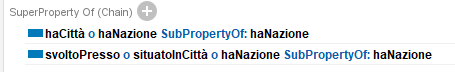
\includegraphics[scale=1]{img/spec_haNazione.png}
       \caption{Modellazione nazione.} 
    \end{center}
\end{figure}
    \item \textbf{haOttenuto}: Indica che un pilota ha ottenuto un piazzamento.
	
    \item \textbf{haPilota}: Indica che un oggetto è associato ad un pilota.
    \item \textbf{cittàNataleDi}: Indica la città natale di un pilota.
    \item \textbf{guidataDa}: Indica che una moto è guidata da un pilota.
    \item \textbf{piazzamentoDi}: Indica che un piazzamento è stato ottenuto da un pilota.
    \item \textbf{seguePilota}: Indica che un capo tecnico segue un pilota.
    \item \textbf{teamDi}: Indica che un team ha un pilota a contratto.
    \item \textbf{tempoDi}: Indica che un tempo è stato segnato da un pilota.
	
    \item \textbf{haSponsor}: Indica che un team o un circuito è associato ad uno sponsor.
    \item \textbf{teamSponsorizzatoDa}: Indica che un team è sponsorizzato da uno sponsor.
    \item \textbf{circuitoSponsorizzatoDa}: Indica che un circuito è sponsorizzato da uno sponsor.
	
    \item \textbf{haStaff}: Indica che un team ha uno staff.
	
    \item \textbf{haTeam}: Indica che ad un soggetto è associato un team.
    \item \textbf{dipendenteDelTeam}: Indica che un membro dello staff dipende da un team.
    \item \textbf{motoDelTeam}: Indica che una moto appartiene ad un team.
    \item \textbf{pilotaDelTeam}: Indica che un pilota corre per un team.
    \item \textbf{sponsorizzaTeam}: Indica che uno sponsor sponsorizza un team.
	
    \item \textbf{inClassificaDi}: Indica che il piazzamento concorre alla classifica di una competizione.
    \item \textbf{lavoraPer}: Indica che uno stuart lavora per un circuito.
    \item \textbf{montatoDa}: Indica che un motore è montato su una moto.
    \item \textbf{produttoreDi}: Indica che un produttore ha costruito una moto (non necessariamente il relativo motore).
    \item \textbf{qualificatoConTempo}: Indica che un posizionamento in qualifica ha un tempo associato.
    \item \textbf{svoltoInCampionato}: Indica che un gran premio è associato ad un campionato.
    \item \textbf{tempoInFP}: Indica che un tempo è associato ad una prova libera.
    \item \textbf{tempoInQ}: Indica che un tempo è associato ad un posizionamento in qualifica.
\end{itemize}

\subsection{Data Properties}
Le data properties consentono di specificare attributi e caratteristiche dei concetti rappresentati dalle classi della nostra ontologia. Di seguito, presentiamo un elenco delle data properties utilizzate da Motology, fornendo una breve spiegazione per ciascuna di esse.\\

\begin{itemize}
\item \textbf{haAnno}: Indica in che anno si svolge un campionato o un gran premio.
\item \textbf{haCilindrata}: Indica la cilindrata di un motore termico.
\item \textbf{haCilindri}: Indica il numero di cilindri di un motore termico.
\item \textbf{haCoppia}: Indica la coppia di un motore.
\item \textbf{haGap}: Indica il gap dal vincitore della gara.
\item \textbf{haLunghezza}: Indica la lunghezza di un circuito.
\item \textbf{haNome}: Indica il nome di un oggetto.
\item \textbf{haNomePersona}: Indica il nome proprio di una persona.
\item \textbf{haNumero}: Indica il numero di un pilota e della sua moto.
\item \textbf{haPosizioneFinale}: Indica la posizione del piazzamento in una competizione.
\item \textbf{haPotenza}: Indica la potenza di un motore.
\item \textbf{haPunti}: Indica i punti ottenuti dal piazzamento in classifica.
\item \textbf{haTempo}: Indica il miglior tempo registrato in una competizione o in un turno di prove.
\item \textbf{haTracciato}: Indica il collegamento all'immagine del tracciato.
\end{itemize}

\section{Regole SWRL}

Di seguito enunceremo le regole implementate in SWRL, per permettere al sistema di derivare informazioni dai dati che già possiede.

\begin{itemize}
  \item \textbf{Regola dello stesso anno}:\\
  
  La regola implica che se un gran premio si svolge in un campionato allora l'anno del GP sarà lo stesso del campionato.\\

  \texttt{moto:svoltoInCampionato(?gp, ?c) \textasciicircum\ moto:haAnno(?c, ?a)\\-> moto:haAnno(?gp, ?a)}

  \item \textbf{Regola del costruttore}:\\
  
  La regola implica che se un team ha degli accordi con uno specifico costruttore allora tutte le moto che ha in scuderia proverranno dallo stesso costruttore.\\

  \texttt{moto:haCostruttoreDelTeam(?t, ?c) \textasciicircum\ moto:haInScuderia(?t, ?m)\\-> moto:costruitaDa(?m, ?c)}

  \item \textbf{Regola del numero}:\\
  
  La regola implica che la moto guidata da un pilota, il quale sceglie il proprio numero, sarà associata al medesimo numero.\\

  \texttt{moto:guidataDa(?m, ?p) \textasciicircum\ moto:haNumero(?p, ?n)\\-> moto:haNumero(?m, ?n)}

  \item \textbf{Regola dello stesso team}:\\
  
  La regola implica che se un pilota fa parte di un team, allora anche la moto che guida rientrerà nella stessa scuderia.\\

  \texttt{moto:pilotaDelTeam(?p, ?t) \textasciicircum\ moto:guidaMoto(?p, ?m)\\-> moto:motoDelTeam(?m, ?t)}

  \item \textbf{Regola del capotecnico}:\\
  
  La regola implica che il capotecnico che segue un pilota apperterrà allo stesso team per il quale gareggia il pilota stesso.\\

  \texttt{moto:pilotaDelTeam(?p, ?t) \textasciicircum\ moto:haCapotecnico(?p, ?c)\\-> moto:dipendenteDelTeam(?c, ?t)}

  \item \textbf{Regola del tempo di piazzamento}:\\
  
  La regola implica che il miglior tempo registrato per il piazzamento in qualifica di un pilota sia stato registrato dal pilota stesso.\\

  \texttt{moto:piazzamentoDi(?piaz, ?pil) \textasciicircum\ moto:qualificatoConTempo(?piaz, ?t)\\-> moto:tempoDi(?t, ?pil)}

  \item \textbf{Regola della leggenda}:\\
  
  La regola implica che se un pilota risulta aver vinto almeno una volta ciascuno dei tre attuali campionati principali, Moto3, Moto2 e MotoGP, allora potrà essere annoverato tra le leggende.\\

  \texttt{moto:Pilota(?p) \textasciicircum\\ moto:haOttenuto(?p, ?piazz1) \textasciicircum\ moto:inClassificaDi(?piazz1, ?ch1) \textasciicircum\ moto:Moto3(?ch1) \textasciicircum\ moto:haPosizioneFinale(?piazz1, 1) \textasciicircum\\ moto:haOttenuto(?p, ?piazz2) \textasciicircum\ moto:inClassificaDi(?piazz2, ?ch2) \textasciicircum\ moto:Moto2(?ch2) \textasciicircum\ moto:haPosizioneFinale(?piazz2, 1) \textasciicircum\\ moto:haOttenuto(?p, ?piazz3) \textasciicircum\ moto:inClassificaDi(?piazz3, ?ch3) \textasciicircum\ moto:MotoGP(?ch3) \textasciicircum\ moto:haPosizioneFinale(?piazz3, 1)\\-> moto:Leggenda(?p)}

\end{itemize}
\chapter{Query ed interrogazioni SPARQL}

In questo capitolo illustriamo alcune query formulate su Motology utilizzando SPARQL, alcune delle quali derivanti da ricerce online legate all'ambito del motomondiale. Occorre precisare che le seguenti query funzionano correttamente solo sull'ontologia contenente anche le triple inferite dal reasoner oltre a quelle modellate in partenza.

\section{Query 1: estrazione delle classifiche}

Con la seguente query è possibile andare a visualizzare tutte le classifiche delle varie competizioni, ordinandole per prime per poi ordinare i vari piazzamenti. \\

\begin{lstlisting}[captionpos=b, caption=Estrazione delle classifiche, label=lst:sparql1,
   basicstyle=\ttfamily,frame=single]
SELECT ?competizione ?pilota ?posizione

WHERE {
	?competizione rdf:type :Competizione .
	?competizione :haInClassifica ?piazzamento .
	?piazzamento :piazzamentoDi ?pilota .
	?piazzamento :haPosizioneFinale ?posizione .
}
ORDER BY ?competizione ?posizione
\end{lstlisting}

\section{Query 2: classifica di una gara}

Con la seguente query è possibile andare a visualizzare la classifica di una specifica gara, in questo caso \texttt{Gara\_1}, ordinata per posizione ottenuta e riportante anche il gap dal vincitore. \\

\begin{lstlisting}[captionpos=b, caption=Classifica di una gara, label=lst:sparql2, basicstyle=\ttfamily,frame=single]
SELECT ?posizione ?pilota (STR(?gap) AS ?Gap) 

WHERE {
	
	?competizione owl:sameAs :Gara_1 .
	?competizione :haInClassifica ?piazzamento .
	?piazzamento :piazzamentoDi ?pilota .
	?piazzamento :haPosizioneFinale ?posizione .
	?piazzamento :haGap ?gap .
}
ORDER BY ?posizione
\end{lstlisting}

\newpage

\section{Query 3: moto e pilota della stessa nazione}

Con la seguente query è possibile andare a visualizzare tutti i piloti che corrono utilizzando una moto prodotta da costruttore riportante la sua stessa nazionalità. Nello specifico si visualizza il nome del pilota, il costruttore e la loro nazione di provenienza.
\\

\begin{lstlisting}[captionpos=b, caption=Moto e pilota della stessa nazione, label=lst:sparql3,
   basicstyle=\ttfamily,frame=single]
SELECT (STR(?pilota) AS ?Pilota) ?costruttore ?nazionalita

WHERE {
	?p rdf:type :Pilota .
	?p :haNomePersona ?pilota .
	?p :haNazione ?nazionalita .
	?p :guidaMoto ?moto .
	?moto :costruitaDa ?costruttore .
	?costruttore :haNazione ?nazionalitaCostruttore .
	?nazionalita owl:sameAs ?nazionalitaCostruttore .
}
\end{lstlisting}


\section{Query 4: numero di gare vinte da ogni pilota}

Con la seguente query è possibile andare a visualizzare per ogni pilota il numero di gare vinte, indipendentemente dal campionato.
\\

\begin{lstlisting}[captionpos=b, caption=Numero di gare vinte da ogni pilota, label=lst:sparql4,
   basicstyle=\ttfamily,frame=single]
SELECT (SAMPLE(STR(?pilota)) AS ?Pilota) (COUNT(?piazzamento) AS ?vittorie) 

WHERE {
	?p rdf:type :Pilota .
	?p :haNomePersona ?pilota .
	?p :haOttenuto ?piazzamento .
	?piazzamento rdf:type :PosizionamentoGara .
	?piazzamento :haPosizioneFinale 1 .	
}
GROUP BY ?p
\end{lstlisting}

\newpage

\section{Query 5: numero di campionati vinti da urbinati}

Con la seguente query è possibile andare a visualizzare per i piloti nati nella città di Urbino il numero di campionati vinti. La query è derivata da quella in \ref{lst:sparql4} con una piccola modifica nella classe presa in considerazione per i piazzamenti.
\\

\begin{lstlisting}[captionpos=b, caption=Numero di campionati vinti da ogni pilota, label=lst:sparql5,
   basicstyle=\ttfamily,frame=single]
SELECT (SAMPLE(STR(?pilota)) AS ?Pilota) (COUNT(?piazzamento) AS ?vittorie) 

WHERE {
	?p rdf:type :Pilota .
	?p :haNomePersona ?pilota .
	?p :natoInCitta ?citta .
	?p :haOttenuto ?piazzamento .
	?piazzamento rdf:type :PosizionamentoCampionato .
	?piazzamento :haPosizioneFinale 1 .	
	FILTER (?citta = :Urbino) .
}
GROUP BY ?p
\end{lstlisting}

\section{Query 6: numero di campionati vinti da ogni team}

Con la seguente query è possibile andare a visualizzare per ogni team il numero di campionati vinti. Anche in questo caso la query è derivata da quella in \ref{lst:sparql4} con una modifica per quanto riguarda l'aggregazione e la gestione dei valori nulli.
\\

\begin{lstlisting}[captionpos=b, caption=Numero di campionati vinti da ogni team, label=lst:sparql6,
   basicstyle=\ttfamily,frame=single]
SELECT (SAMPLE(?team) AS ?Team) (COUNT(?piazzamento) AS ?Vittorie) 

WHERE {
	?team rdf:type :Team .
	OPTIONAL{
	?p rdf:type :Pilota .
	?p :haOttenuto ?piazzamento .
	?piazzamento rdf:type :PosizionamentoCampionato .
	?piazzamento :haPosizioneFinale 1 .	
	?p :pilotaDelTeam ?team .
	}
}
GROUP BY ?team 
ORDER BY DESC (?Vittorie)
\end{lstlisting}

\newpage

\section{Query 7: piazzamenti "patriottici"}

Con la seguente query è possibile andare a visualizzare tutti i piazzamenti ottenuti dai piloti nei propri circuiti di casa, ovvero con la stessa nazione associata, solo nel caso in cui corrano con una moto di un costruttore della stesso paese.
\\

\begin{lstlisting}[captionpos=b, caption=Piazzamenti "patriottici", label=lst:sparql7,
   basicstyle=\ttfamily,frame=single]
SELECT (STR(?pilota) AS ?Pilota) ?costruttore (STR(?nomeCircuito) AS ?Circuito) ?nazionalita ?posizione

WHERE {
	?p rdf:type :Pilota .
	?p :haNomePersona ?pilota .
	?p :haNazione ?nazionalita .
	?p :guidaMoto ?moto .
	?moto :costruitaDa ?costruttore .
	?costruttore :haNazione ?nazionalita .
	?p :haOttenuto ?piazzamento .
	?piazzamento rdf:type :PosizionamentoGara .
	?piazzamento :haPosizioneFinale ?posizione .
	?piazzamento :inClassificaDi ?gara .
	?gara :corsaInGP ?gp .
	?gp :haNazione ?nazionalita .
	?gp :svoltoPresso ?circuito .
	?circuito :haNome ?nomeCircuito .
}
\end{lstlisting}

\section{Query 8: numero di piloti per team}

Con la seguente query è possibile andare a visualizzare tutti i team presenti e il loro numero di piloti a contratto.
\\

\begin{lstlisting}[captionpos=b, caption=Numero di piloti per team, label=lst:sparql8,
   basicstyle=\ttfamily,frame=single]
SELECT (SAMPLE(?t) AS ?team) (COUNT(?p) AS ?NumeroPiloti)

WHERE {
	?t a :Team .
	OPTIONAL {
		?t :teamDi ?p .
		}
}
GROUP BY ?t
ORDER BY DESC (?NumeroPiloti)
\end{lstlisting}

\newpage

\section{Query 9: numero di campionati vinti per nazione}

Con la seguente query è possibile andare a visualizzare il numero di campionati vinti da ogni nazione.
\\

\begin{lstlisting}[captionpos=b, caption=Numero di campionati vinti per nazione, label=lst:sparql9,
   basicstyle=\ttfamily,frame=single]
SELECT (SAMPLE(?n) AS ?nazione) (COUNT(?piazzamento) AS ?campionatiVinti) 

WHERE {
	?p a :Pilota .
	?p :haOttenuto ?piazzamento .
	?piazzamento a :PosizionamentoCampionato .
	?piazzamento :haPosizioneFinale 1 .	
	?p :haNazione ?n .
}
GROUP BY ?n
\end{lstlisting}

\chapter{Conclusioni}

Il progetto ci ha permesso di comprendere quanto il web semantico rappresenti e rappresenterà in futuro uno strumento indispensabile in molteplici ambiti, per ottenere informazioni anche complesse con la semplicità di un interrogazione ad un sistema interconnesso, collaborativo ed interoperabile, superando tutte quelle che sono le attuali limitazioni del web.
\\\\
Molte informazioni ricavate tramite query effettuate su Motology stessa senza l'impiego del web semantico sarebbero state svariati minuti di ricerca ed integrazione di dati presenti su motori di ricerca tradizionali, riteniamo pertanto che l'obiettivo di partenza sia stato pienamente soddisfatto dal nostro sistema.

\section{Sviluppi futuri}
Gli sviluppi futuri del progetto sono numerosi e riguardano diversi campi: 

\begin{itemize}
\item Web semantico: l'ontologia può facilmente essere impiegata in altri progetti, sia di natura più generale che più dettagliata, inoltre potrebbe essere estesa a tutti gli sport motociclistici (superbike, enduro etc.), potrebbe essere integrata con dati dei veicoli in modo da ottenere informazioni più dettagliate riguardo i singoli componenti della moto etc.
\item Machine learning: un ontologia di questo tipo potrebbe essere utilizzata in progetti di machine learning per allenare modelli predittivi analizzando trend che possono emergere dallo studio dei dati interconnessi da Motology.

\end{itemize}

\end{document}
